% --- Header --- %
\documentclass[review]{elsarticle}
%\usepackage{authblk}
%\usepackage[utf8]{inputenc}
%\usepackage[english]{babel}
%\usepackage[style=alphabetic]{biblatex}
%\addbibresource{references.bib} % include citations/references
%\usepackage{listings}
%\usepackage{multirow}
%\usepackage{geometry}
%\usepackage{gensymb}
%\usepackage{booktabs}
%\usepackage{mathtools} 
%\usepackage{lipsum}
%\usepackage{color}
%\usepackage{graphicx}
%\usepackage{ragged2e}
%\usepackage{pgfplots}
%\graphicspath{figures/}

% --- Front --- %
\begin{document}
\title{Applications of computer-vision for agricultural implement feedback and control}

\begin{abstract}
Management of organic row crops requires frequent in-field
operations. Depending on the extent of soil conservation practices, 
weed control necessitates tillage operations. Strip-tillage and
cultivator implements require precise guidance systems to
assure proper positioning of the working tools. Legacy systems have
made use of mechanical guiding rods, however such
systems perform poorly during the earliest stages of crop growth.
Modern techniques based on RTK GPS are available commercially but are
prohibitively expensive for small-scale operations.
Therefore, the objective of this study was to develop a low-cost CCD 
camera system which is capable of supplementing the mechanical row detection during inter-row cultivation.
A computer-vision guidance system was developed for the Intel Atom 
architecture to interface with an electro-hydraulic steering hitch system.
Two redundant CCD cameras were mounted to the cultivator toolbar
in-line with crop rows to obtain a video stream of the plants passing beneath the implement.
The OpenCV platform was used to develop an algorithm for identifying
the lateral offset of the plant rows and adjust the hydraulic steering
accordingly via PID control. The computer-vision guidance system was
tested successfully without GPS RTK assistance at travel speeds of 6,
8, 10, and 12 km/h in corn and soybean fields under varying ambient
light and crop conditions.
\end{abstract}

\section{Introduction}
Unlike conventional farming where herbicide application is the primary
method for weed prevention, organic farmers must use tillage
implements such as inter-row cultivators. Inter-row cultivation is a
field operation which requires precise control of the implement in
order to maximize the tillage area without causing damage to the
crops. Often, cultivation is conducted at speeds of up to 12 km/h with
an error tolerance of $\pm$5 cm. Many organic farmers are not equipped
with RTK-guided tillage implements and prefer to use older,
mechanically-guided systems. A common method for mechanically-guided
cultivators employs guiding rods (also known as
brushes) which are mounted to a rotating voltage divider
(\ref{guiding_rods}). These rods make contact with the crop stems and their
position approximates that of the crop row. The resulting reference
signal is fed to a hydraulic control system which adjusts the steering
mechanism of the implement accordingly. Although these
mechanically-guided systems are rugged and maintainable, the guiding
rods perform poorly with seedlings. During the early stages of growth
guiding rods have the potential to cause damage to the crop or lose
track of the row, forcing operators to travel at speeds of less than 6
km/h. To address this issue, modern systems implement non-contact
detection methods, such as a secondary RTK GPS antennae or cameras, to
estimate the lateral offset of the cultivator.

\begin{figure}
  \centering
  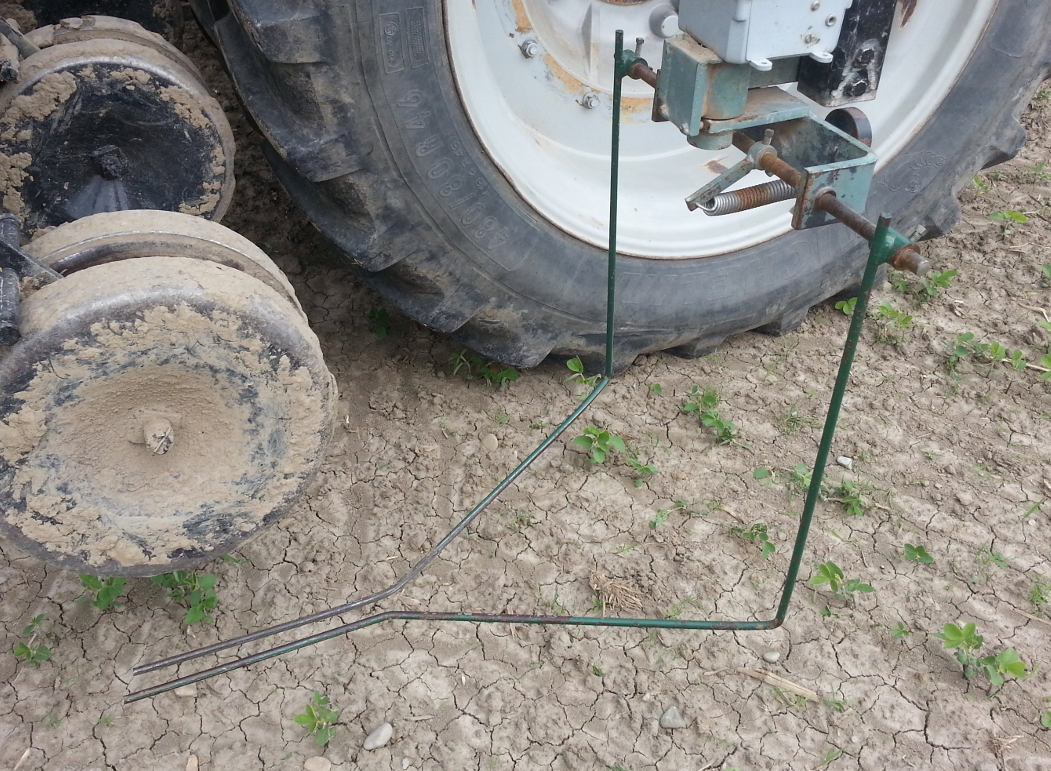
\includegraphics[width=0.8\textwidth,natwidth=610,natheight=642]{guiding_rods.jpg}
  \caption{Mechanical guiding rods.}
  \label{fig:guiding_rods}
\end{figure}

The objective of this study was to develop a low-cost, embedded system
which extends computer-vision row detection functionality to existing
electro-hydraulic implement guidance systems.  To be considered
effective, the system should be capable of 4 cm precision 95 percent of the 
time for travel speeds up to 12 km/h and for crops up to 20 cm in
height.

\section{Literature Review}
Demand for high precision tractor control has produced significant
research interest over the past two decades. Studies by Hague et
al., Kise et al., and Astrand et al. have demonstrated that by 
capturing a video stream of the crop rows passing by tractor, the 
lateral offset of vehicle relative to the crop rows can be estimated
with a high degree of consistency. The lateral offset detected in this manner
has also been shown to be an effective input for actuating agricultural 
implements.

Several different computer-vision methodologies have been proposed for 
detecting the offset of the crop row such as stereo-vision, distribution
of crop foliage, Hough transform, and band-pass analysis.

In order to identify the location of the crop row, t

In order to identify the location of the crop row, the distribution of
plant foliage within the captured images must be determined, a process
known as segmentation. During this process, varying ambient light
conditions is one of the major limiting factors for successfully
implementing computer-vision guidance for weed control. Variations in
the ambient color temperature occur naturally with changes in weather
and time of day, as well as with the particular camera model being
used. Additionally, irregular lighting intensity, also known as
non-diffuse lighting, in the camera’s field of view, such as from
shadows cast by the cultivator, is also a major concern. Non-diffuse
lighting results in greater difference in the intensity of pixels and
reduces the effectiveness when differentiating between color hues.
 
Several different image filtering methods can be utilized for
segmentating of plants from soil. Using unfiltered RGB data is not
commonly employed due to the high correlation between the three
channels. Therefore, conversion to an alternate color-space is often
advantagous for plant identification. An approach proposed by Meyer et
al. (1998) demonstrates a contrast filter known as Excess Green (ExG)
calculated using the following equation:

\begin{equation}
    ExG = \displaystyle\sum_{j=1}^{H} \displaystyle\sum_{i=1}^{W} \frac{G_{i,j}-R_{i,j}}{R_{i,j} + G_{i,j} + B_{i,j}}
\end{equation}
\begin{flushleft}
where $n_{x}$ = image width (pixels); $n_{y}$ = image height (pixels).
\end{flushleft}

The transformed image is passed through a low-pass filter to remove
bright spots before a constant threshold value of 20 on a scale of 0
to 255 is applied. This method was tested in diffuse natural light
conditions in a greenhouse environment between 11:30am and 12:30pm and
resulted in a 100 successful rate of discrimination between plants and
soil.

Alternative approaches have utilized HSV transform

\begin{figure}
  \centering
  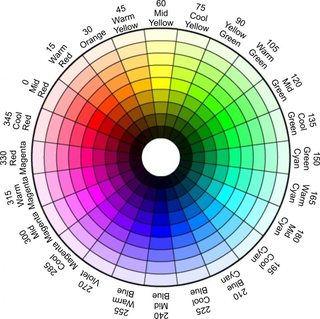
\includegraphics[width=0.8\textwidth,natwidth=610,natheight=642]{hsv.jpg}
  \caption{HSV Transform (360 degree).}
  \label{fig:hsv}
\end{figure}

After segmentation of the plants within the image, it is necessary to
determine the lateral offset of the crop row. Methods for determining
the lateral offset can be grouped into two classes based on whether
the camera’s angle of inclination is either equal to zero, or greater
than zero; these classes are referred to as orthogonal or perspective,
respectfully. 

\begin{figure}
  \centering
  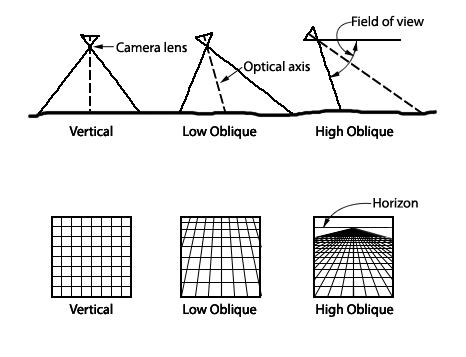
\includegraphics[width=0.8\textwidth,natwidth=610,natheight=642]{oblique_projection.jpg}
  \caption{Perspective vs. orthogonal viewing angles.}
  \label{fig:projection}
\end{figure}

Orthogonal methods rely on a camera which faces vertically downward
and is directly aligned with a single crop row of the cultivator. A
basic approach proposed by Olson et al. (1995) for detecting the
lateral offset of the crop relies on taking the sum of the pixel
elements grey values in the direction of travel. The resulting curve
represents the likelihood of the row’s position for each x-index
within the image. To isolate the most probable offset, two separate
methods were compared: 1) a least squares regression of a sinusoidal
wave, and 2) a Fourier Fast Transform (FFT) low-pass filter. Both
filtration methods were effective in cereals to within an error of 10
mm, but performed poorly on sugar beets due to their
characteristically large leaf volume. In a similar study by Slaughter
et al. (1995), an algorithm for detecting the lateral offset of the
row using individual segmentation of plants in the image was
proposed. For each plant, a histogram of the intensities was
calculated which was then used to find the median offset of each
plant. If a plant’s median was significantly different than the other
plants in the image, it was considered a weed and disregarded. The row
offset was then calculated based on the medians of the remaining
plants. This method was tested on lettuce and tomatoes for use with a
band sprayer operating at 8 km/h and performed successfully with
standard error of 9 mm and within 12 mm 95\% of the time.

Conversely, perspective methods rely on a camera with a positive angle
of inclination with multiple rows in the field of view. One approach
for perspective guidance utilizes the Hough Line Transform (HLT)
algorithm to detect linear rows in cauliflower, sugar beets, and
wide-spaced wheat. In a study by Pla et al. (1997), a system using HLT
performed with an error of 18 mm, which was considered sufficient by
the researchers. A similar perspective approach using a band-pass
filter proposed by Hague et al. (2001) based on prior knowledge of the
spacing of the crop rows was developed for use on cereals and
beets. Supported by the British Beet Research Organization the
developed system was capable of 3 cm precision at speeds of up to 10
km/h. The project was considered highly successful and was
commercialized in 2001 in partnership with Garford Farm Machinery and
Robodome Electronics under the name RoboCrop.

When comparing the orthogonal and perspective methods, both have
advantages and disadvantages. The perspective approach is less
sensitive to missing plants and high weed density. However,
perspective methods rely on prior knowledge of the crop spacing and
linear rows with low curvature. Comparatively, orthogonal systems
optimize resolution, in pixels-per-centimeter, and require very only
basic calibration. Lens distortion is an issue for perspective
systems. To compensate for increased subject distance, perspective
methods require a higher resolution camera, resulting in greater
computational requirements and costs. The reduced field of view for
orthogonal systems is a concern when there are significant gaps in the
crop rows. To address the issues inherent to the orthogonal approach,
a system with two or more cameras may provide sufficient redundancy.

Actuation of the implement position can be achieved by several
methods, such as vehicular steering, pivoting hitches, side-shift
hitches, or stabilizer steering. Of these, vehicular steering has
received tremendous interest however is not applicable in all
environments. Some providers have produced mountable steering but no
computer-vision versions have been successfully produced. Pivoting
hitch systems have also been manufactured. For light cultivation, the
side-shift style hitch has been demonstrated to be effective. However,
this method causes problems when mounted to a heavy cultivator (deep
harrows or coulters) due to “jumping”, i.e. the effect of the hitch
shifting the tractor. To address this requires either removing tools
or dramatically increasing the weight of the tractor, both of which
are undesirable to the farmer. Stabilizer steering has applications in
heavier tillage.

\begin{equation}
  D = F_{i} \left[ A + B(S) + C(S^2) \right] W * d
  \label{eq:soil_resistance}
\end{equation}

A hydraulic hitch positional control system can be expressed as a
linear system. The output is the lateral error of the vehicle relative
to the crop row and the input is the position of the steering
mechanism. Additionally, state-information of the system is required,
and it is assumed the angular speed is constant and travel speed is
within acceptable bounds. To control this system, the voltage signal
to the electrohydraulic steering can be modulated to adjust the
lateral position of the cultivator.

\begin{equation}
  F_x = V - \rho\theta(sin \beta sin \alpha \sin \theta + cos \alpha +
  cos \theta)
  \label{eq:horizontal_velocity}
\end{equation}
\begin{flushleft}
where $V_x$ is the velocity in the x-axis, $\theta$ is the yaw of the
disc, $\alpha$ is the pitch of the
disc, $\beta$ is the roll of the disc, $\rho$ is the distance from
the axis of rotation of the disc to the given point of the working surface.
\end{flushleft}

\section{Methodology}
For field evaluation, a twelve row Hiniker cultivator equipped with a
Sukup Auto-Guidance system mounted to a Fendt Vario 850 was used
throughout the testing period. The cultivator toolbar was configured
to a row-spacing of 30 inches. Steering actuation of the cultivator
was achieved via two 75 cm stabilizers mounted 165 cm behind the
cultivator toolbar and spaced 147.8 cm apart. The hydraulic actuation
of the stabilizers had maximum angular travel of $\pm$1.31 rad and angular
velocity of 0.4 rad/s.

\begin{figure}
  \centering
  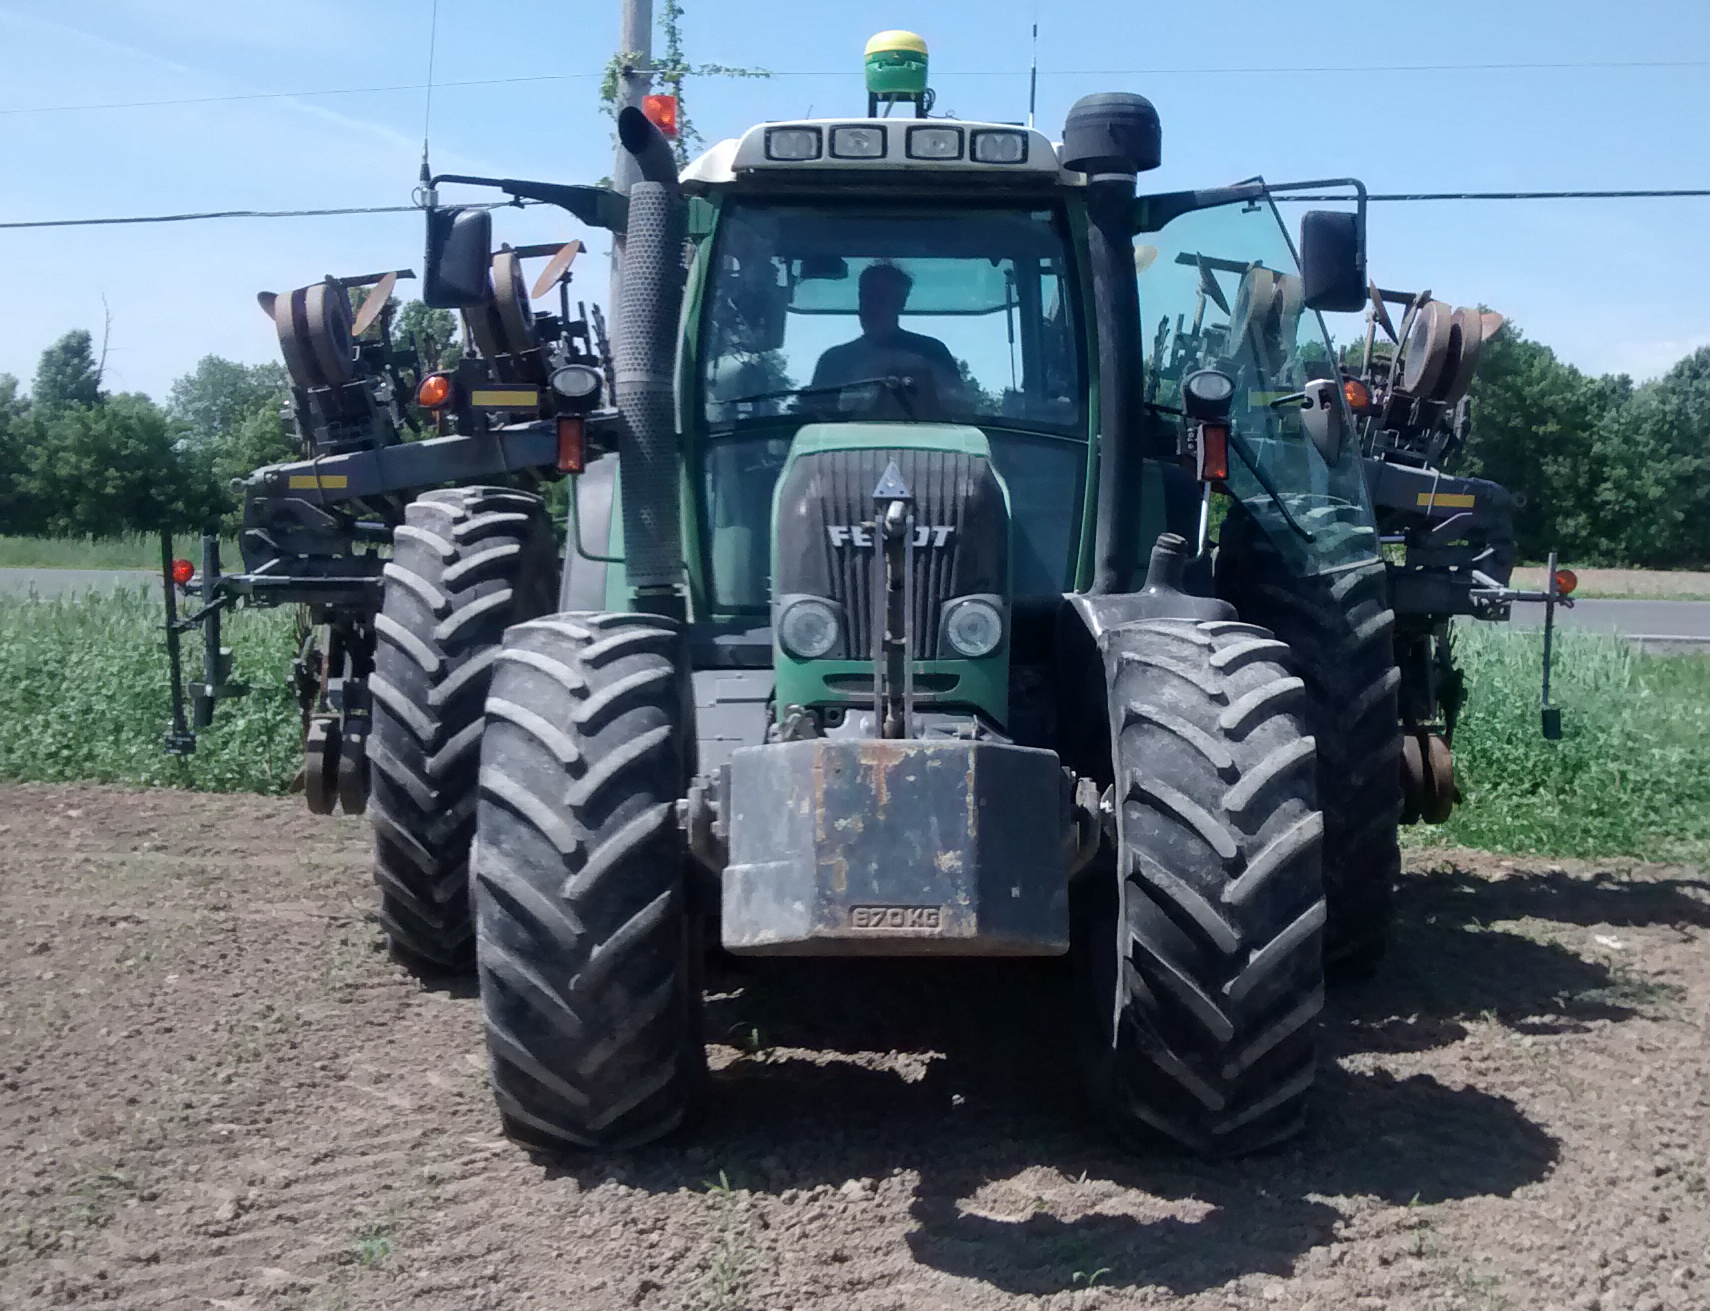
\includegraphics[width=0.8\textwidth,natwidth=610,natheight=642]{fendt_front.jpg}
  \caption{Diagram of the cultivator implement mounted to the tractor.}
\end{figure}

The computer-vision guidance system was installed alongside the
existing mechanical guidance system to act as a replacement for the
guiding rod potentiometer. The remaining components of the Sukup
Auto-Guide system, including the electrohydraulic controller,
center-pivot potentiometer, manual adjustment inputs, and hydraulic
solenoids, were unmodified. This configuration allowed easily
switching between the two modes of operation during field trials.

\begin{figure}
  \centering
  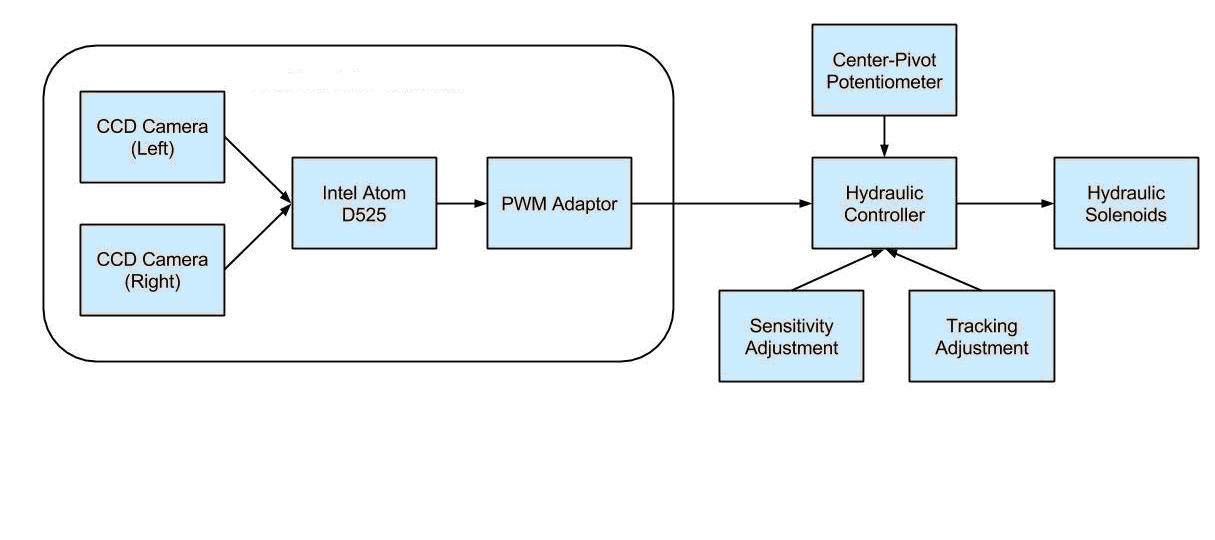
\includegraphics[width=0.8\textwidth,natwidth=610,natheight=642]{agcv_diagram.png}
  \caption{Diagram of the computer-vision system integrated with hydraulic controller.}
\end{figure}

Images of the plants passing beneath the cultivator are captured by
two weather-proof CCD cameras mounted via C-brackets to he toolbar. 
In a compromise between the orthogonal and perspective
methods, the two cameras were mounted at a 30$^{\circ}$ inclination from
vertical and a subject depth of 100 cm. This approach provides
additional longitudinal field of view without significantly
contributing to image distortion. To provide row estimation redundancy
in the event of regions of high weed density or gaps in the crop rows,
the two cameras were installed on the 3rd and 9th row of the
cultivator.

An embedded Linux system based on the Debian 7.8 operating system
(Linux Kernel 3.2) was developed for the Intel Atom D525
architecture. A 1.8GHz processor was used, with a 32 GB SSD, and 1 GB
of RAM (Jetway). A run-time application was developed for the system
using the Python programming language (v. 2.7.6) which operated as a
local microwebserver. A high-speed database server (MongoDB 32-bit)
was implemented for ultra-low latency storage and retrieval of
data. This robust platform provided sufficient computing power for
real-time image analysis at a relatively low cost. To generate the
output voltage signal of the control system, an
ATmega328P microcontroller was used as an 8-bit PWM generator. The
microcontroller was integrated as a Universal Serial Bus (USB)
peripheral device with the microprocessor as the host. 

Additionally a graphical user interface was developed to aid user
operation which allows the operator to check the performance of the
guidance system in real-time.

\subsection{Plant Segmentation}
Video of the crop rows were captured in real-time from the two CCD
cameras. The cameras used for this study had a native resolution and
frame-rate of 640x480 and 25 frames-per-second, respectively. However,
were hardware downscaled to a resolution of 320x240 and 16
frames-per-second. After capturing an image, the image matrix was
transformed from the Red-Green-Blue (RGB) color-space to the
de-correlated Hue-Saturation-Value (HSV) color-space in order to
simplify band-pass filtering operations (Equations \ref{eq:rgb2h} to \ref{eq:rgb2v}).

\begin{equation}
  H_{i,j} =
  \begin{cases}
    60 * \frac{G-B}{V_{i,j}-min(R_{i,j},G_{i,j},B_{i,j})}  & \quad \text{if } V = R \\
    120 + 60 * \frac{B-R}{V_{i,j}-min(R_{i,j},G_{i,j},B_{i,j})}  & \quad \text{if } V = G \\
    240 + 60 * \frac{R-G}{V_{i,j}-min(R_{i,j},G_{i,j},B_{i,j})}  & \quad \text{if } V = B \\
  \end{cases}
  \label{eq:rgb2h}
\end{equation}

\begin{equation}
  S_{i,j} = 
  \begin{cases}
    \frac{V_{i,j}-min(R_{i,j},G_{i,j},B_{i,j})}{V_{i,j}}  & \quad \text{if } V \neq 0 \\
    0  & \quad \text{else}\\
  \end{cases}
  \label{eq:rgb2s}
\end{equation}

\begin{equation}
  V_{i,j} = max(R_{i,j},G_{i,j},B_{i,j})
  \label{eq:rgb2v}
\end{equation}

After transforming the image to the HSV color-space, a band-pass plant
detection filter (BPPD) was applied to isolate pixels which could
represent plant foliage. This filter selects for pixels with hue
ranging from yellow-green to blue-green, saturation above the mean
saturation, and value (i.e. brightness) between the extremes of under-
and over-exposed. Threshold values were determined empirically using a
training set of sample images in varying light and crop
conditions. During this process, it was observed that the cameras
experienced significant blue-shifting of crop foliage in very bright
or low light, so the upper threshold for hue was set well into the
cyan-blue region. This change did not have any noticeable negative
impact on performance due to the relative lack of blue-tones in soil.
\begin{equation}
  P_{n}(C) = A_{nN} + (nN \text{mod} 1) \times (A_{\lfloor nN \rfloor + 1}-A_{nN})
  \label{eq:percentile}
\end{equation}
\begin{flushleft}
where $n$ is the percentile of the  sorted array $A$ of $C$ of length N.
\end{flushleft}

This is the band-pass algorithm which was used:

\begin{equation}
BPPD_{i,j} =
  \begin{cases}
    1  & \quad \text{if } H_{min}<H_{i,j}<H_{max}(S) \bigwedge P_{k}(S)< S_{i,j} <P_{l}(S) \bigwedge P_{m}(V)< V_{i,j}<P_{n}(V)\text{ }\\
    0  & \quad \text{else}\\
  \end{cases}
  \label{eq:bppd}
\end{equation}
\begin{flushleft}
where $H_{min}=45$ (yellow-green), $H_{max}=105$ (blue-green).
\end{flushleft}

The BPPD filter utilizes the linear interpolation percentile function
to calculate the upper and lower thresholds of the Value and
Saturation bands. This approach eliminates the need for static limits,
reducing false-positive classification of pixels as green under
varying lighting conditions. As a final post-processing step,
morphological opening with a 3 by 3 kernel was applied to the BPPD
mask to reduce any remaining noise while preserving the structure of
crop foliage:

\begin{equation}
M = BPPD \otimes
\begin{bmatrix}
       1 & 1 & 1 \\
       1 & 1 & 1 \\
       1 & 1 & 1
     \end{bmatrix}
\label{eq:morph_opening}
\end{equation}
\begin{flushleft}
where K is a 3 by 3 kernel.
\end{flushleft}

This three step process is computationally non-intensive, yet produces
sufficient segmentation in diverse lighting conditions. Notably, the
percentile-based band-pass filters of saturation and intensity
produced reliable masks in scenarios of extreme exposure and shadows.

\begin{figure}
  \centering
  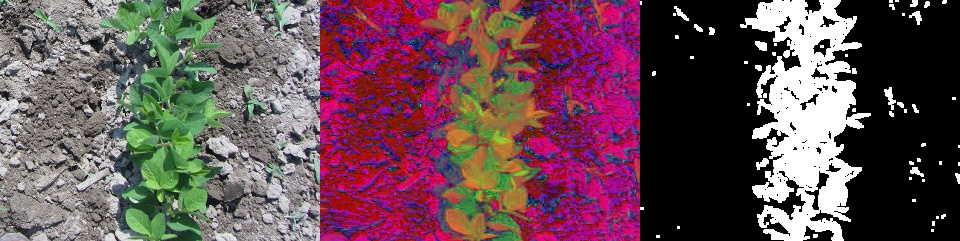
\includegraphics[width=0.8\textwidth,natwidth=610,natheight=642]{bppd_normal.jpg}
  \caption{BPPD applied to image of soy row.}
  \label{fig:bppd_normal}
\end{figure}

\begin{figure}
  \centering
  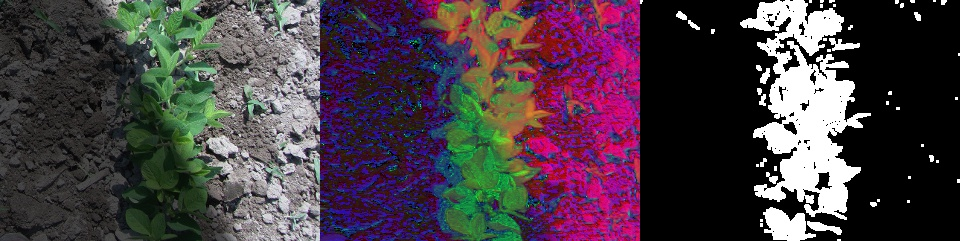
\includegraphics[width=0.8\textwidth,natwidth=610,natheight=642]{bppd_shadow.jpg}
  \caption{BPPD Shadow}
  \label{fig:bppd_shadow}
\end{figure}

\subsection{Row Estimation}
After the plant foliage mask (M) has been produced, the column
summation of the mask was calculated in the direction of travel,
resulting in an array (C) representing the lateral distribution of
plant foliage within the image. 

\begin{equation}
  C_{i} = \displaystyle\sum_{j=1}^{H} M_{i,j}
  \label{eq:col_sum}
\end{equation}
\begin{flushleft}
where H=240
\end{flushleft}

Indices of the C-array with low values suggest bare-soil, moderate
values suggest sparsely distributed weeds, and higher values suggest
presence of the crop row due to the longitudinal alignment of the
plant foliage. Using this distribution, the centroid of the crop row
was estimated by applying a high-pass filter to select for indices
which are significantly greater than others: 

\begin{equation}
  p_{i} =
  \begin{cases}
    i & \quad \text{if } C_{i} \geq P_{\alpha}(C) \\
    0 & \quad \text{else} \\
  \end{cases}
  \label{eq:p_threshold}
\end{equation}
\begin{flushleft}
where $\alpha$=0.95
\end{flushleft}

The array (p) consists of all indices of the image which are most
likely to represent the crop row. The estimated centroid of the crop
row was determined by taking the weighted mean of the probable
indices, where weight of each index was the normalized value of its
corresponding column summation:

\begin{equation}
    x = \frac{\displaystyle\sum_{i=1}^{N} p_{i} \times
      C_{i}}{\displaystyle\sum_{j=1}^{N} C_{p_{i}}} - \frac{W}{2}
  \label{eq:centroid}
\end{equation}
\begin{flushleft}
where $N$ is the number of elements in $p$ and $x$ is the position the
estimated centroid in pixels.
\end{flushleft}

To compensate for errors in the detection process inherent to single
camera systems, the row centroid estimation process was repeated for
each image, producing two column summation arrays ($C_{1}$ and $C_{2}$) and two
estimated row centroids ($x_{1}$ and $x_{2}$). After calculating the estimated
row centroid for each camera, the centroid and column summation values
are compared to determine the final estimated offset of the crop row:

\begin{equation}
  e = 
  \begin{cases}
    mean(x_{1},x_{2})  & \quad \text{if } |x_{1}-x_{2}| \leq  \epsilon\\
    argmax(C_{1},C_{2})  & \quad  \\
  \end{cases}
  \label{eq:camera_selection}
\end{equation}
\begin{flushleft}
where $\epsilon$ is the maximum acceptable error tolerance, $W$ is the width of
the camera in pixels. 
\end{flushleft}

This approach prioritizes centroid estimations which are in agreeance
and in the event of disagreeance between the two cameras the dominant
centroid was taken as the row. This provided a simplistic means for
reducing errors due to weeds. For the sake of performance evaluation,
the error in pixels may be converted to centimeters using the
relationship between the cameras’ field-of-view of 64 cm, measured
width-wise along the center-line, at a subject depth of 100 cm. For a
resolution of 320 px in width, this results in a resolution of 0.2 cm/px.

\begin{equation}
  x = \frac{We}{w}
  \label{eq:px2mm}
\end{equation}
\begin{flushleft}
where $e$ is the error, $W$ is the field-of-view of the camera (in
centimeters), $w$ is the camera width (in pixels).
\end{flushleft}

This is what it looks like:

\begin{figure}
  \centering
  % 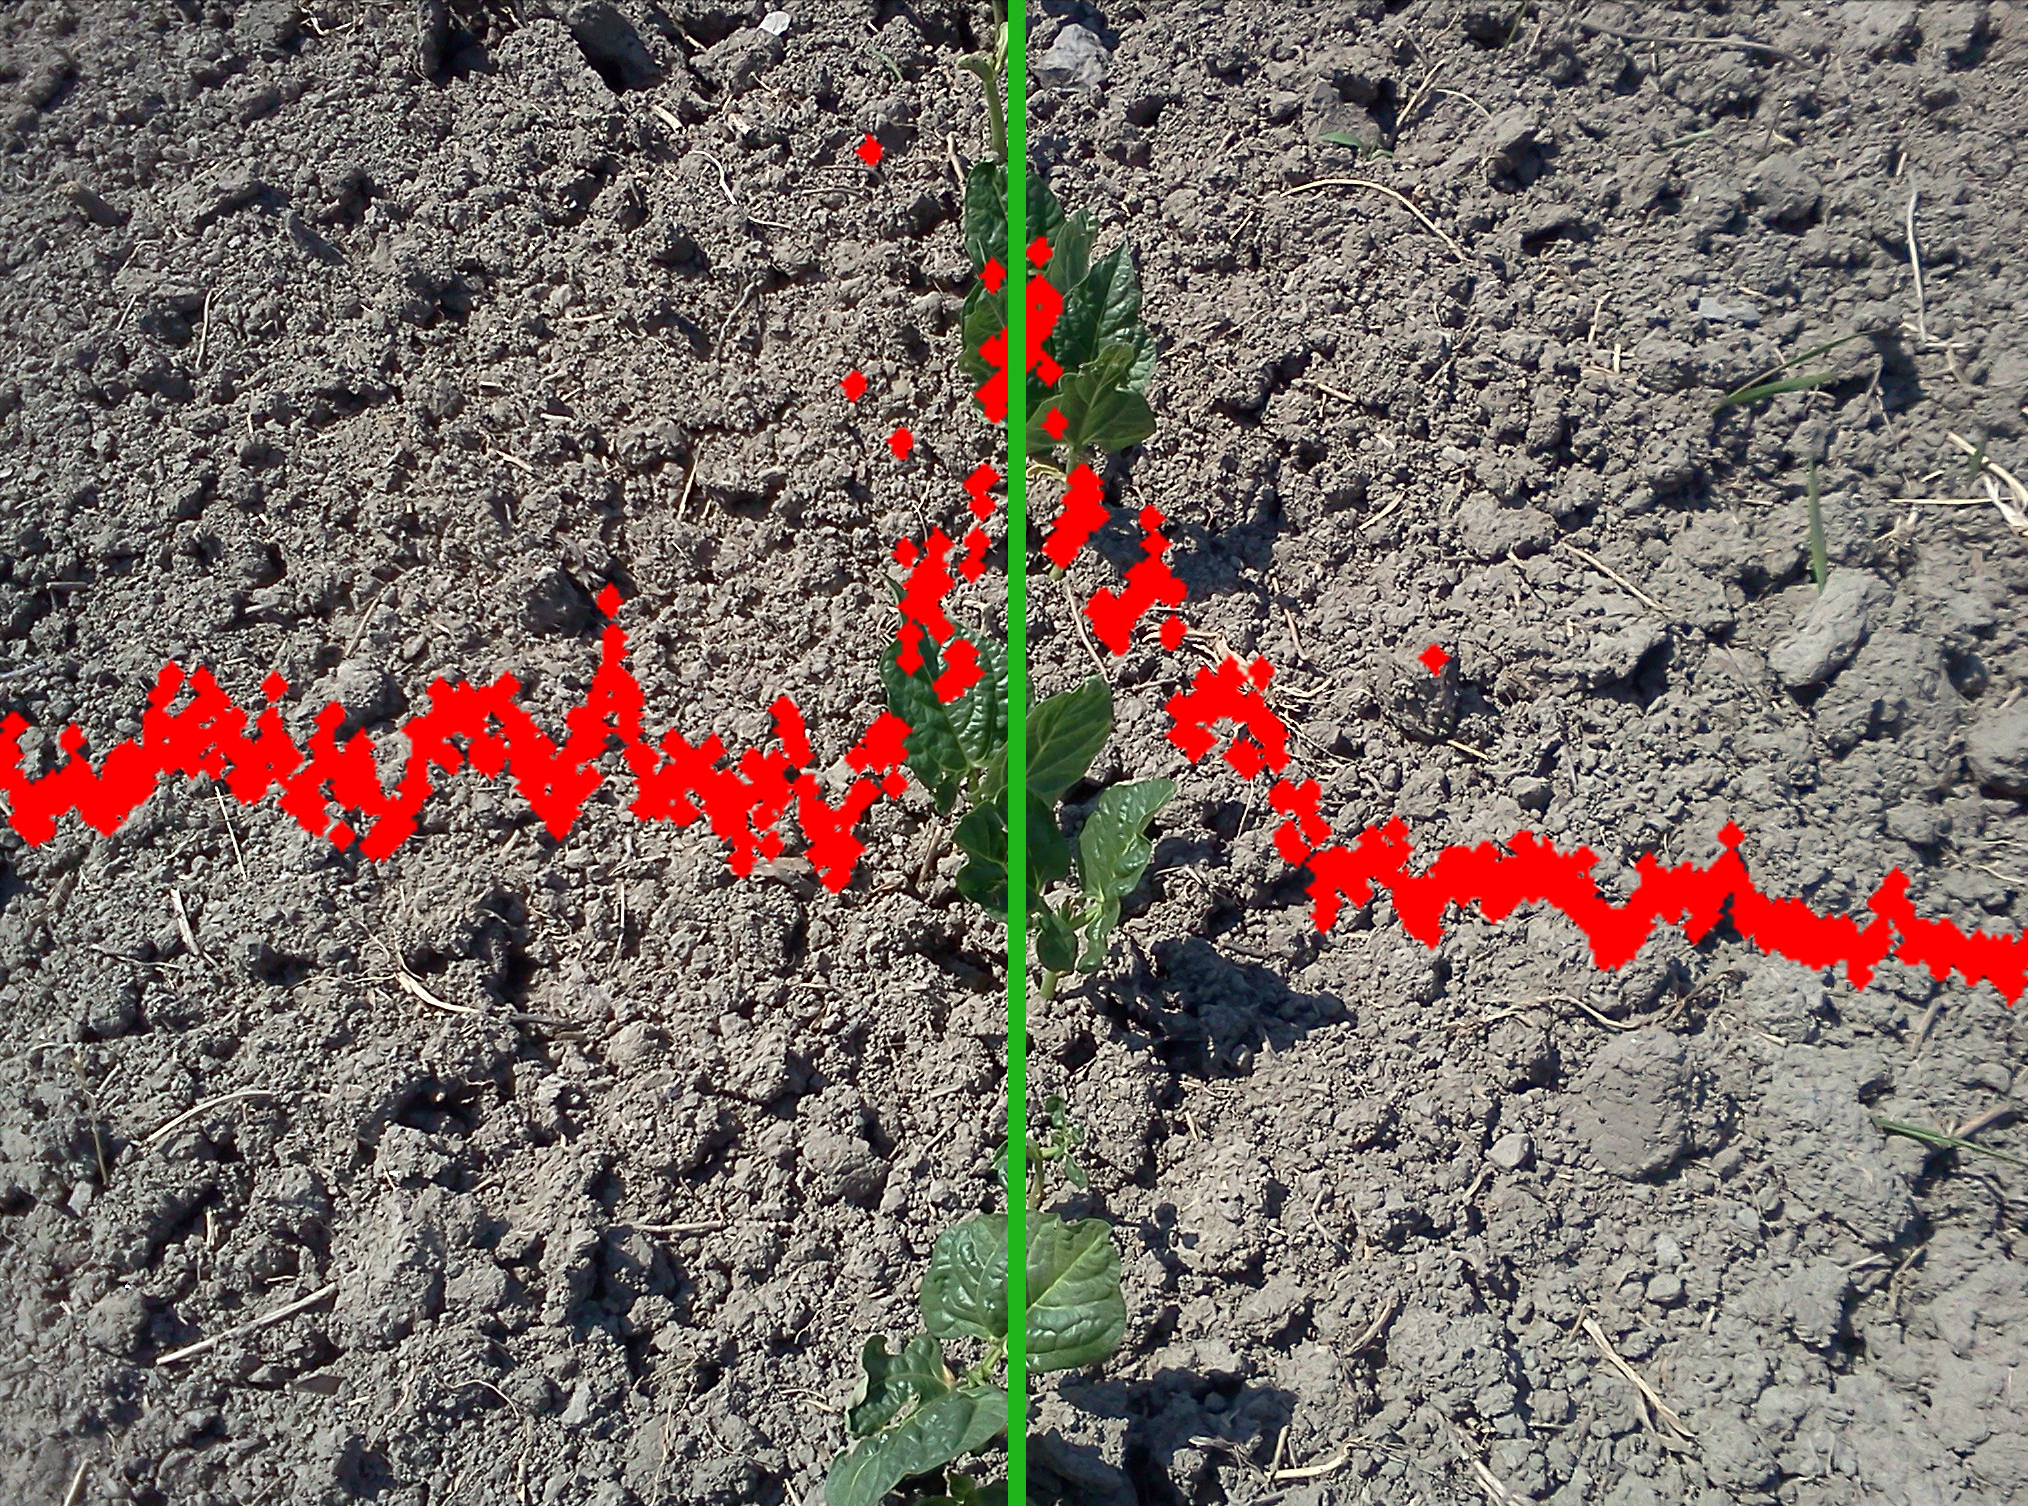
\includegraphics[scale=0.4]{row_estimation.jpg}
  \caption{Demonstration of offset detection.}
  \label{fig:row_estimation}
\end{figure}

\subsection{Electro-hydraulic Control}
The rotary stabilizer mechanism was operated via bang-bang hydraulic
solenoid controller whose actuation was based on the voltage
differential between the feedback signal from the row detection
system, i.e. the guiding rods or computer-vision module, and the
potentiometer mounted to the rotary mechanism on the hitch. 
To generate a smooth output signal, a signal conditioning based on a
Proportional-Integral-Derivative (PID) feed-back controller was
implemented. Coefficients were initially chosen to provide similar
response to that of the guiding rods and were subsequently modified by
trial and error.
\begin{equation}
    u(t) = K_{P}e_{t} + \frac{K_{I}}{N}\displaystyle\sum_i^N \left[
      e_{t-i} \right] +
    \frac{K_{D}}{M}\displaystyle\sum_{i=1}^M \left[e_{t-i}-e_{t-i-1}\right]
  \label{eq:pid}
\end{equation}
\begin{flushleft}
where $K_{P}=1.0$, $K_{I}=4.0$, $K_{D}=0.5$, $N=15$ is the number of integral samples,
$M=3$ is the number of differential samples.
\end{flushleft}

\begin{figure}
  \centering
  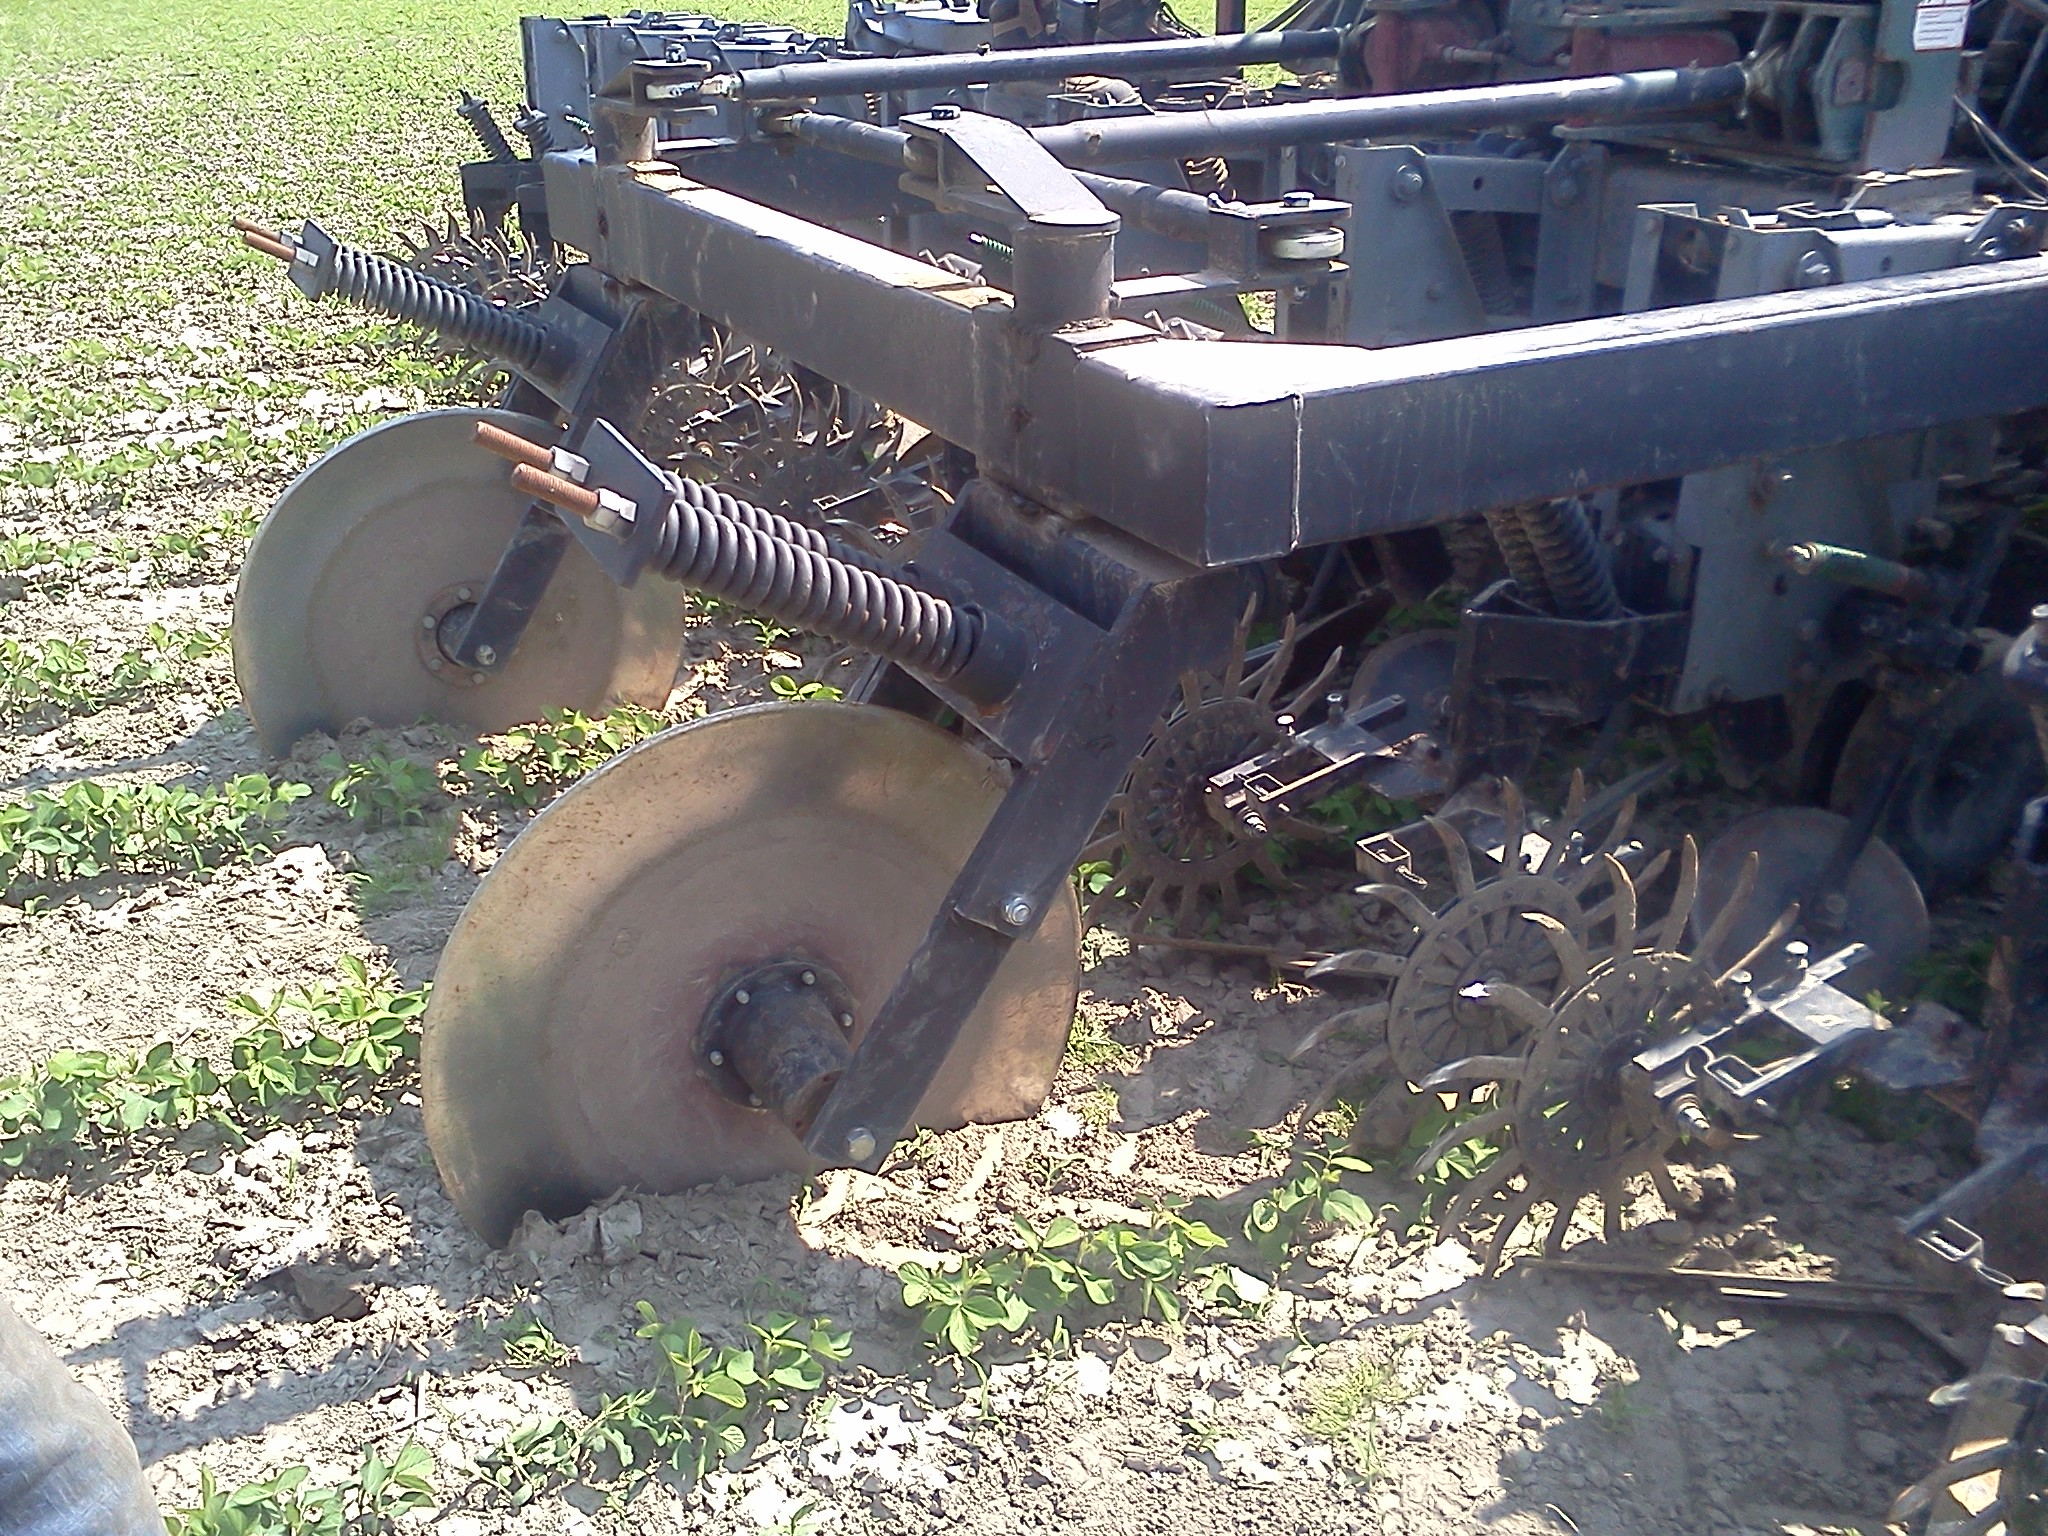
\includegraphics[scale=0.1,natwidth=610,natheight=642]{stabilizers.jpg}
  \caption{Rotating stabilizers}
  \label{fig:stabilizers}
\end{figure}

The output value was transmitted via a weatherproof (IP68) USB
connection to the microcontroller which was interfaced with the
hydraulic solenoid controller. The microcontroller generates an analog
output signal via pulse-width modulation (PWM) to produce a voltage
range from 0.0 V to 5.0$\pm$0.05 V. However, the operating range of the
Sukup Auto-Guide system is from 0.10$\pm$0.02V to 8.0$\pm$0.02V with a fixed
supply voltage of 9.70$\pm$0.02V. To account for this discrepancy, the PWM
output range was scaled linearly and a logic level converter (LLC)
circuit was used to rescale and shift the PWM signal to the required
range.

\begin{equation}
  w = 
  \begin{cases}
    0 & \quad \text{if } u \leq 0 \\
    2^{R-1} & \quad \text{if } u \geq 2^{R-1}\\
    (u +2^{R-2})\times\left[\frac{V_{max}}{V_{HV}}+\frac{V_{min}}{V_{LV}}\right] & \quad \text{else} \\
  \end{cases}
  \label{eq:v_out}
\end{equation}
\begin{flushleft}
where $V_{min}=0.10$, $V_{max}=8.00$, $V_{HV}=9.70$, $V_{LV}=5.0$
\end{flushleft}

\begin{equation}
  V_{hydraulic} = \frac{w}{2^{R-1}} \times V_{HV} + V_{min}
  \label{eq:v_out}
\end{equation}
\begin{flushleft}
where $V_{min}=0.10$, $V_{max}=8.00$, $V_{HV}=9.70$, $V_{LV}=5.0$
\end{flushleft}

To produce this output, a signal condition circuit was employed making
use of a MOSFET logici-level converter. This allows the system to
output a voltage using PWM to systems with different voltage
requirements.

\begin{figure}
  \centering
  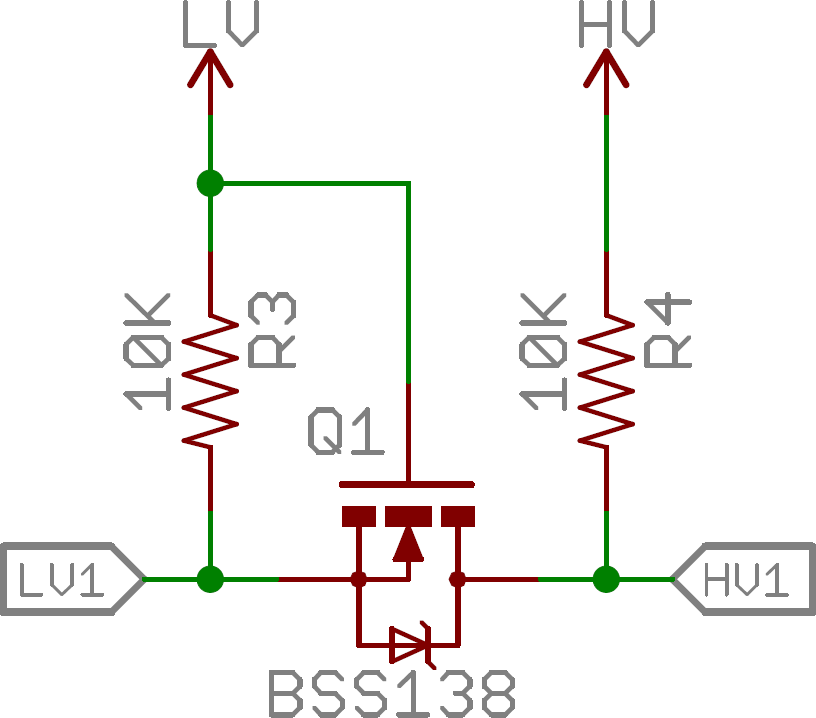
\includegraphics[scale=0.3,natwidth=610,natheight=642]{signal_conditioning.png}
  \caption{Rotating stabilizers}
  \label{fig:signal_conditioning}
\end{figure}

This final output voltage represents the desired set-point for angle
of the steering stabilizers to be reached by hydraulic solenoid
controller. The mapping between output voltage and position was found
to be a linear, second order system, with saturation.

\begin{equation}
  \frac{d^2}{dt^2}x + 2\zeta\omega_{n}\frac{d}{dt}x + \omega_{n}^2 Kx = 0 
  \label{eq:v_out}
\end{equation}
where $K=0.3275$ rad/V at a sensitivity setting of 10.

\subsection{Calibration}
At the beginning of each day of field trials, a camera calibration
procedure was followed to ensure proper alignment of the cameras: (1)
the cultivator was aligned with the crop rows which was verified by
measurements with a tape measure at the working tools; (2) lateral
adjustments were made to the camera bracket to ensure the vertical
center-line of each camera was aligned with the crop row; (3) vertical
adjustments made to the camera bracket to ensure a subject depth of
100 cm from the camera lens to the soil surface.

Additionally, the Sukup Auto-Guide system provides basic user tuning
in the form of sensitivity and tracking adjustment inputs. The
sensitivity adjustment effectively changes the mapping between voltage
and radial resolution of the stabilizers, with a range of 1 to 10
resulting in mappings from 0.1350 rad/V to 0.3275 rad/V,
respectively. Similarly, the tracking adjustment offsets the zero
position of the stabilizers on a scale of -3 to +3 corresponding to
-0.435 rad to +0.435 rad, respectively. Therefore, at the beginning of
each set of trials the following settings were ensured: (1) the
sensitivity was set to 10 out of 10, and (2) the tracking adjustment
was set to 0.

\subsection{Field Trials}
Field tests of the system took place over the summer of 2014 from June
to August on straight-drilled corn and soybean crops. Only organic
cultivars were considered for this study, therefore no pesticides were
applied to the fields and weeds were present during testing. All
fields used during testing were maintained by Agri-Fusion 2000 Inc., a
4000 ha organic farming operation in St-Polycarpe, Quebec. Trials were
classified into four stages of crop development: $\le$10 cm, 10 - 15
cm, 15 - 20 cm, and $\ge$20 cm. For each run, five representative
locations along the row were selected and the height of the crop from
the soil surface was observed using a tape measure, and the resulting
average determined the height stage of the trial. To determine the
reliability of the two systems at differing speeds of operation,
trials were conducted at four approximate travel speeds: 6, 8, 10, and
12 km/h. The travel speed of the tractor was set via the automatic
speed controller of the vehicle.

\section{Results}
\begin{table}[h]
  \centering
  \caption{RMSE and 95$^{th}$ Percentile
    with respect to crop-stage.} 
  \scalebox{0.6}{
    \begin{tabular}{lcccccccc}
      \toprule
      \multirow{2}[10]{*} & \multicolumn{4}{c}{RMSE (cm)} &
      \multicolumn{4}{c}{95$^{th}$ Percentile (cm)} \\
      \cmidrule(1r){2-5} \cmidrule(1r){6-9}  
      & $\le$10 cm & 10-15 cm & 15-20 cm & $\ge$20 cm & $\le$10 cm & 10-15 cm & 15-20 cm & $\ge$20 cm \\
      \midrule
      Computer-vision & 0.50 $\pm$ 0.1 & 19.36 $\pm$ 0.1 & 63.69 $\pm$ 0.1 & 65.67 $\pm$ 0.1 & 38.86 $\pm$ 0.1 & 38.9 $\pm$ 0.1 & 145.55 $\pm$ 0.1 & 143.69 $\pm$ 0.1 \\
      Guiding rods & 21.33 $\pm$ 0.1 & 20.92 $\pm$ 0.1 & 66.33 $\pm$ 0.1 & 66.15 $\pm$ 0.1 & 6.53 $\pm$ 0.1 & 6.00 $\pm$ 0.1 & 3.84 $\pm$ 0.1 & 3.50 $\pm$ 0.1 \\
      \bottomrule  
    \end{tabular}}
  \label{table:travel_speed}
\end{table}

\begin{table}[h]
  \centering
  \caption{RMSE and 95$^{th}$ Percentile with respect to travel speed.}
  \scalebox{0.6}{
    \begin{tabular}{lcccccccc}
      \toprule
      \multirow{2}[10]{*} & \multicolumn{4}{c}{RMSE (cm)} &
      \multicolumn{4}{c}{95$^{th}$ Percentile (cm)} \\
      \cmidrule(1r){2-5} \cmidrule(1r){6-9}  
      & 6 km/h & 8 km/h & 10 km/h & 12 km/h & 6 km/h & 8 km/h & 10 km/h & 12 km/h \\
      \midrule
      Computer-vision & 1.78 $\pm$ 0.1 & 1.9 $\pm$ 0.1 & 2.3 $\pm$ 0.1 & 2.8 $\pm$ 0.1 & 38.86 $\pm$ 0.1 & 38.9 $\pm$ 0.1 & 145.55 $\pm$ 0.1 & 143.69 $\pm$ 0.1 \\
      Guiding rods & 21.33 $\pm$ 0.1 & 20.92 $\pm$ 0.1 & 66.33 $\pm$ 0.1 & 66.15 $\pm$ 0.1 & 38.39 $\pm$ 0.1 & 38.35 $\pm$ 0.1 & 133.34 $\pm$ 0.1 & 4.0 $\pm$ 0.1 \\
      \bottomrule  
    \end{tabular}}
 \label{table:travel_speed}
\end{table}

\section{Discussion}
With respect to RMSE, the two systems performed comparatively, with an
average RMSE of less than 3.5 cm for both the computer-vision and the
guiding rod systems for all crop stages \ref{table:travel_speed}. However, with
respect to the 95th percentile, usage of the guiding rods resulted in
greater error than the computer-vision system for crops at the $\le$10 cm,
10-15 cm, and 15-20 cm stages. Notably, the guiding rods resulted in
an average 95th percentile of 6.57 cm and 6.53 cm for the $\le$10 cm and
10-15 cm stages, respectively. Comparatively, the computer-vision
system had an average 95th percentile of less than 4 cm for all four
crop stages. The accuracy of the guiding rods increased dramatically
as the plants matured, resulting in a significant decline in average
95th percentile and average RMSE at the 15-20 cm and $\ge$20 cm
stages. The computer-vision system showed significantly lower error
than the guiding rods for crop stages less than 20 cm in height, but a
slight increase in error for plants greater than 20 cm. 

There was no apparent correlation between error and travel speed for
both systems, either with respect to RMSE or 95th percentile. Notably,
the computer vision guidance system outperformed the mechanical system
at all travel speeds; however, this affect is likely due to the
interaction with crop height, not travel speed.

\subsection{Future Improvements}
Due to the fact that the cameras used for this study were intended for
security applications, the cameras were designed for usage in a wide
range of ambient lighting. Specifically, the photosensor of the
cameras was sensitive to infrared (IR) light and featured a built-in
array of 24 IR LEDs. Although this feature theoretically extended the
daily hours of operation, IR-sensitivity proved to have a negative
affect on color-quality under intense ambient light, i.e. $\ge$50000 Lux,
resulting in over-exposure and blue-shifting of green tones in the HSV
color-space. To correct this, applying contrast-limited adaptive
histogram equalization (CLAHE) as pre-processing prior to the BPPD
filter may reduce the negative affects of IR-sensitivity without
requiring hardware changes (e.g. non-IR sensitive cameras or usage of
an IR filtering lens).

In this study, since row offsets were determined by analyzing the
plant foliage mask in the direction of travel with a relatively small
subject distance, no perspective or radial (also referred to as
lens-distortion) correction was implemented. However for alternate
usage cases, e.g. cameras aligned at the mid-point between rows, it
would be necessary for perspective and lens-distortion correction to
be implemented. Due to the nature of how these systems are installed,
a versatile method for in-field camera calibration demonstrated by Lee
et al. in 2002 can be utilized. This method makes use of a
checkerboard pattern which is placed in the camera’s field of view. An
image is captured and the positions of the corners are
identified. Using the known size of the squares, the calibration
coefficients can be calculated which can be used on new images to
rectilinearize the image, thus correcting for perspective and radial
distortion.

This study focused on a rotating stabilizer hydraulic steering system
and therefore the orientation of the crop rows relative to the
cultivator (and by extension the cameras) was effectively
orthogonal. This approach is appropriate for rotating stabilizer and
center-shift steering systems; however several commercially available
hydraulic steering system designs make use of a pivoting hitch system
(\ref{fig:pivoting_hitch}).

\begin{figure}
  \centering
  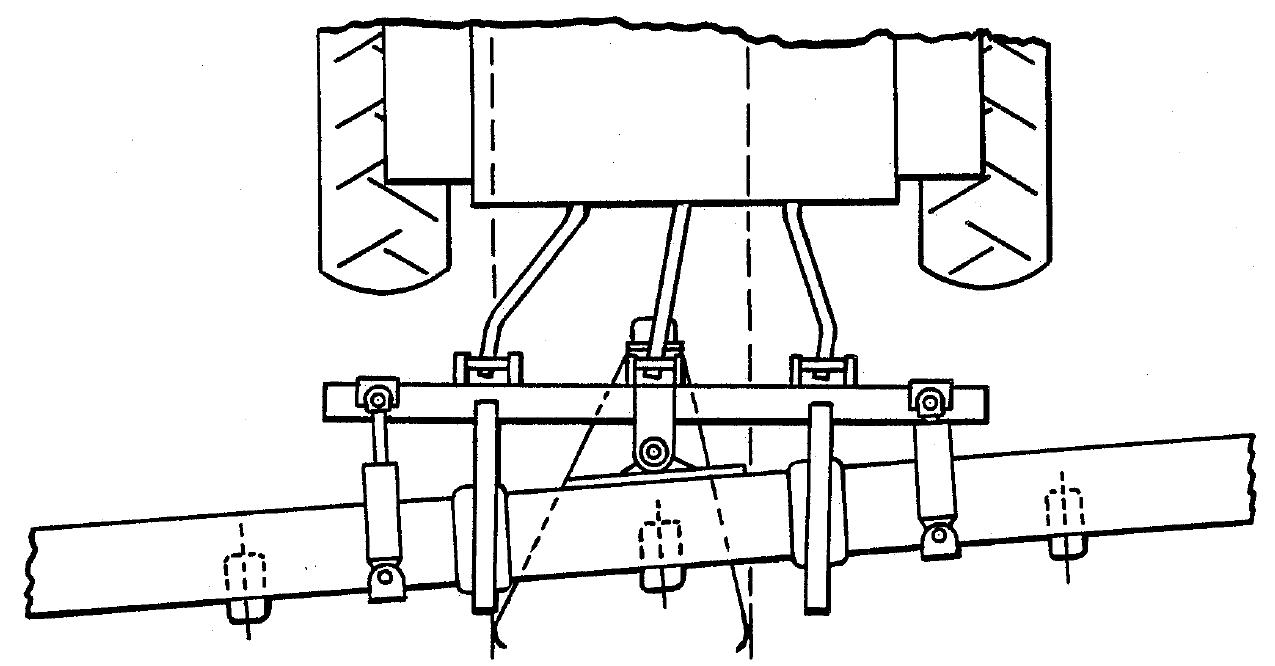
\includegraphics[width=0.8\textwidth,natwidth=610,natheight=642]{pivoting_hitch.png}
  \caption{Pivoting hitch hydraulic steering system.}
  \label{fig:pivoting_hitch}
\end{figure}

Such pivoting hitch steering systems may rotate the cultivator toolbar
as much as $\pm5$ degrees and would therefore significantly
reduce the accuracy of row estimation. To compensate for this effect,
knowledge of the camera orientation and its position relative to the
pivot point is required. Motion estimation of the cameras using
feature-based keypoint tracking may be a robust solution which does
not require integration with the hitch controller and is therefore
system-agnostic.

\begin{figure}
  \centering
  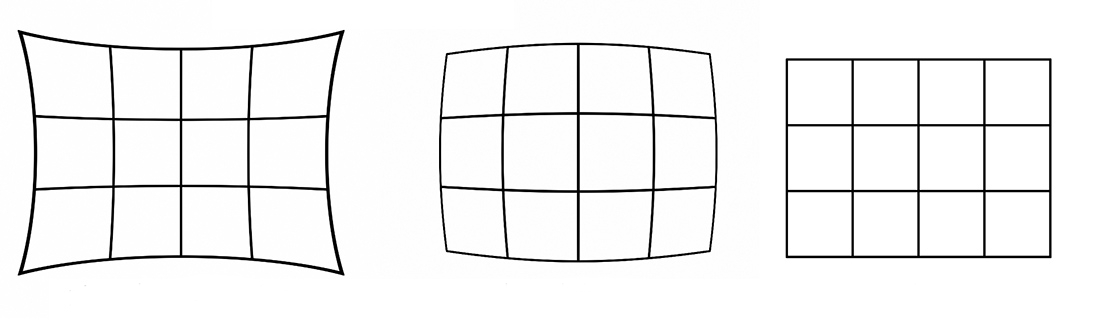
\includegraphics[width=0.8\textwidth,natwidth=610,natheight=642]{lens_distortion.jpg}
  \caption{Lens distortion}
  \label{fig:distortion}
\end{figure}

Although manual inputs are maintained by interfacing with a hydraulic
controller, adaptive control of the system could be implemented. Tunig
of the PID coefficients via reinforcement learning techniques, such as
Q-Learning, may be highly applicable to this manner of control system.

A method for implementing such a adaptive controller has been
explored. By treating subsets of the response as actions, the
response of the system can optimized in real-time. 

\begin{equation}
  Q = 
  \label{eq:qlearning}
\end{equation}
\begin{flushleft}
Cost function for evaluating actions.
\end{flushleft}

Additional feedback mechanisms, such as the vehicles travel-speed, may
also prove useful in adjusting the system response.

\section{Conclusion}
The BPPD method worked well in various lighting conditions and crop conditions.
The computer-vision system achieved an average 95th percentile of <
4.0 cm for all crop stages, and significantly outperformed the guiding
rods at the earliest stages of <10 cm and 10-15 cm. Calibration
procedure was simple

\subsection{Acknowledgements}
This study was supported in part by funding provided through the
National Science and Engineering Research of Canada (NSERC) Engage
program with assistance from Jean Cantin of the Quebec Ministry of
Agriculture, Fisheries and Food.
